%%%%%%%%%%%%%%%%%%%%%%%%%%%%%%%%%%%%%%%%%%%%%%%%%%%%%%%%%%%%%%%%%%%%%%%%%%%%%%%%%%%%%%%%%%%%%%%%%%%%%%%%%%%%%%%%%%%%%%%%%%%%%%%%%%%%%%%%%%%%%%%%%%%%%%%%%%%%%%%%%%%%%%%%%%%%%%

\UC{Visualizzazione carrello}
\begin{figure}[H]
    \centering
    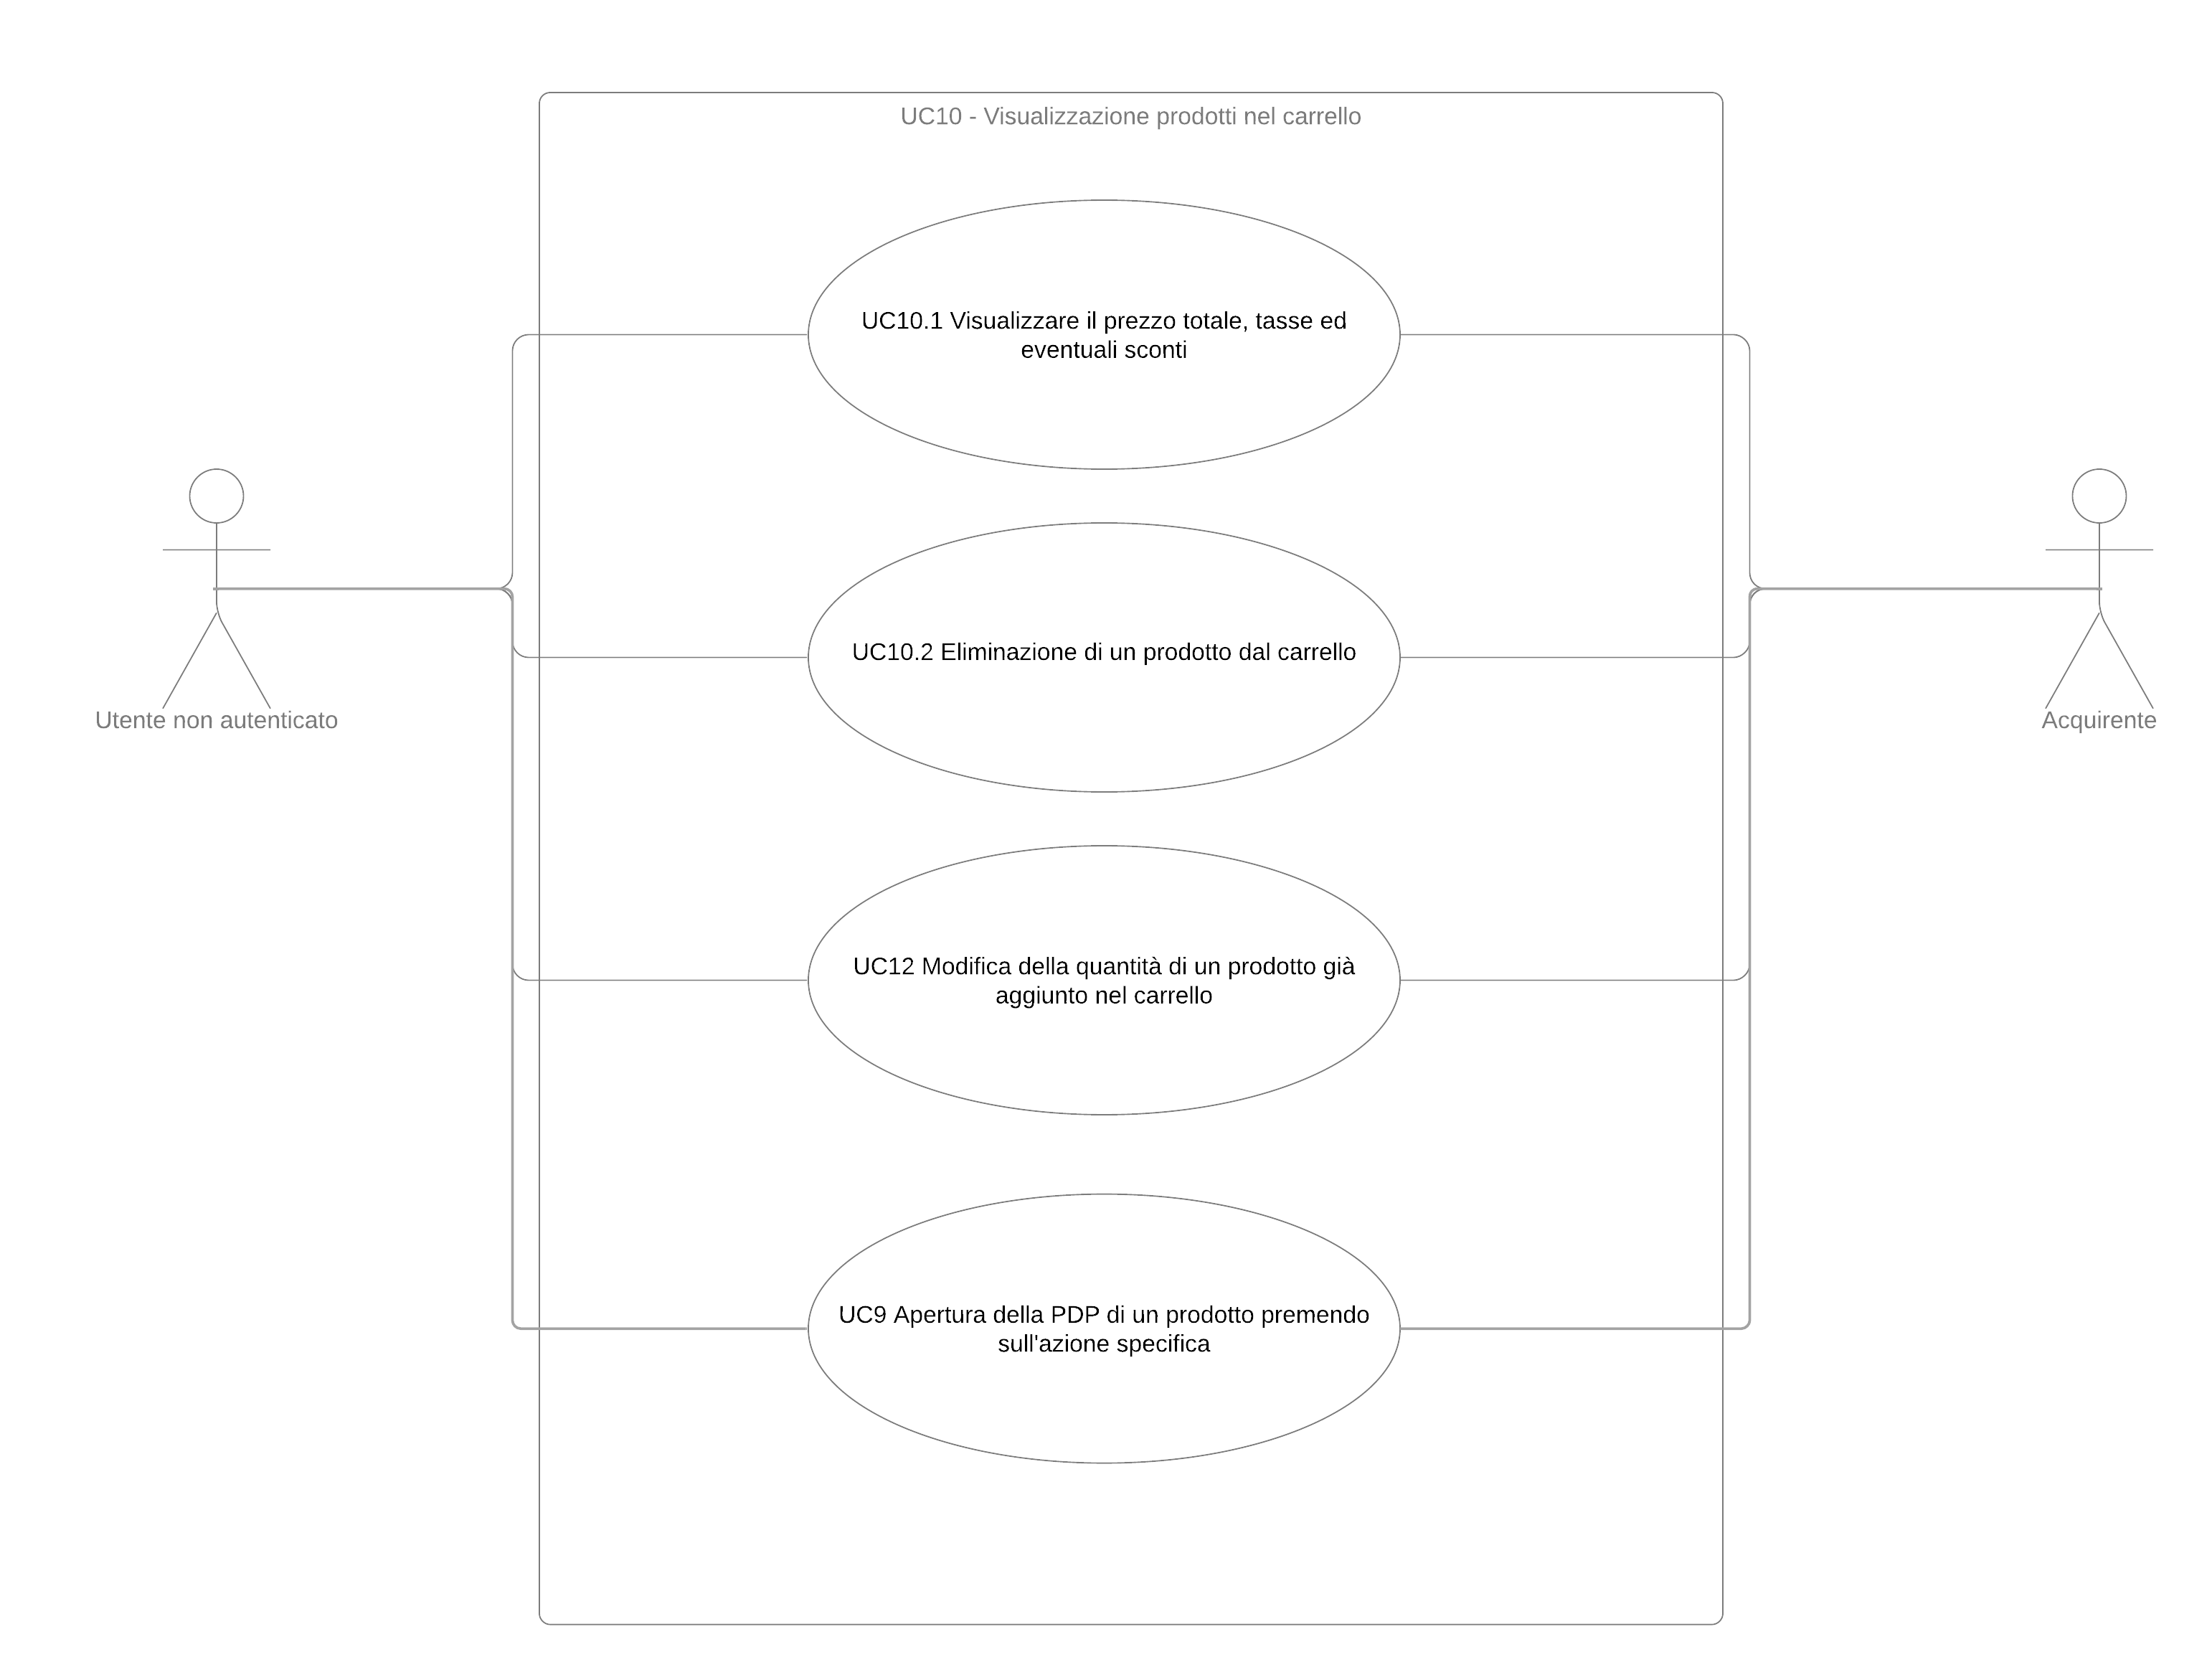
\includegraphics[width=\textwidth]{Immagini/DiagrammiUC/UC10VisualizzazioneProdottiNelCarrello.png}
    \caption{Diagramma di \actualUC: Visualizzazione prodotti nel carrello} 
    \label{fig:VisualizzazioneProdottiNelCarrello}
\end{figure}
L'utente vuole visualizzare il proprio carrello.
\begin{itemize}
    \item \textbf{Attori primari:} acquirente o utente non autenticato;
    \item \textbf{Precondizione:} l'attore si trova in una qualunque schermata della piattaforma;
    \item \textbf{Postcondizione:} l'attore visualizza il proprio carrello con l'elenco dei prodotti presenti;
    \item \textbf{Scenario principale:} l'attore seleziona la funzionalità per passare al carrello, da qui può:
    \begin{itemize}
        \item Visualizzare i prodotti presenti con il prezzo totale, tasse ed eventuali sconti;
        \item (UC) - Eliminare un prodotto dal carrello;
        \item (UC) - Modificare la quantità di un prodotto;
        \item (UC) - Aprire la PDP di un prodotto premendo sull'azione specifica;
        \item (UC) - Procedere al checkout.
    \end{itemize}
    \item \textbf{Scenario alternativo:} non ci sono prodotti all'interno del carrello, verrà visualizzato il messaggio "Carrello vuoto" e sarà data la possibilità all'attore di andare alla schermata principale per iniziare gli acquisti.
\end{itemize}

%%%%%%%%%%%%%%%%%%%%%%%%%%%%%%%%%%%%%%%%%%%%%%%%%%%%%%%%%%%%%%%%%%%%%%%%%%%%%%%%%%%%%%%%%%%%%%%%%%%%%%%%%%%%%%%%%%%%%%%%%%%%%%%%%%%%%%%%%%%%%%%%%%%%%%%%%%%%%%%%%%%%%%%%%%%%%%

\UC{Eliminazione di un prodotto dal carrello}
L'acquirente o l'utente non autenticato può eliminare un prodotto che ha inserito nel carrello.
\begin{itemize}
    \item \textbf{Attori Primari:} acquirente o utente non autenticato;
    \item \textbf{Precondizione:} l'attore è nella pagina del carrello e ha inserito almeno un prodotto;
    \item \textbf{Postcondizione:} l'attore ha rimosso totalmente il prodotto dal carrello;
    \item \textbf{Scenario Principale:} l'attore non vuole più ordinare un prodotto che ha aggiunto nel carrello e, per farlo, svolge le seguenti operazioni:
    \begin{itemize}
        \item clicca sull'azione di eliminazione del prodotto dal carrello;
        \item il prodotto viene rimosso dal carrello.
    \end{itemize}
\end{itemize}

%%%%%%%%%%%%%%%%%%%%%%%%%%%%%%%%%%%%%%%%%%%%%%%%%%%%%%%%%%%%%%%%%%%%%%%%%%%%%%%%%%%%%%%%%%%%%%%%%%%%%%%%%%%%%%%%%%%%%%%%%%%%%%%%%%%%%%%%%%%%%%%%%%%%%%%%%%%%%%%%%%%%%%%%%%%%%%

% \UC{Aggiunta del prodotto al carrello}
% \begin{figure}[H]
%     \centering
%     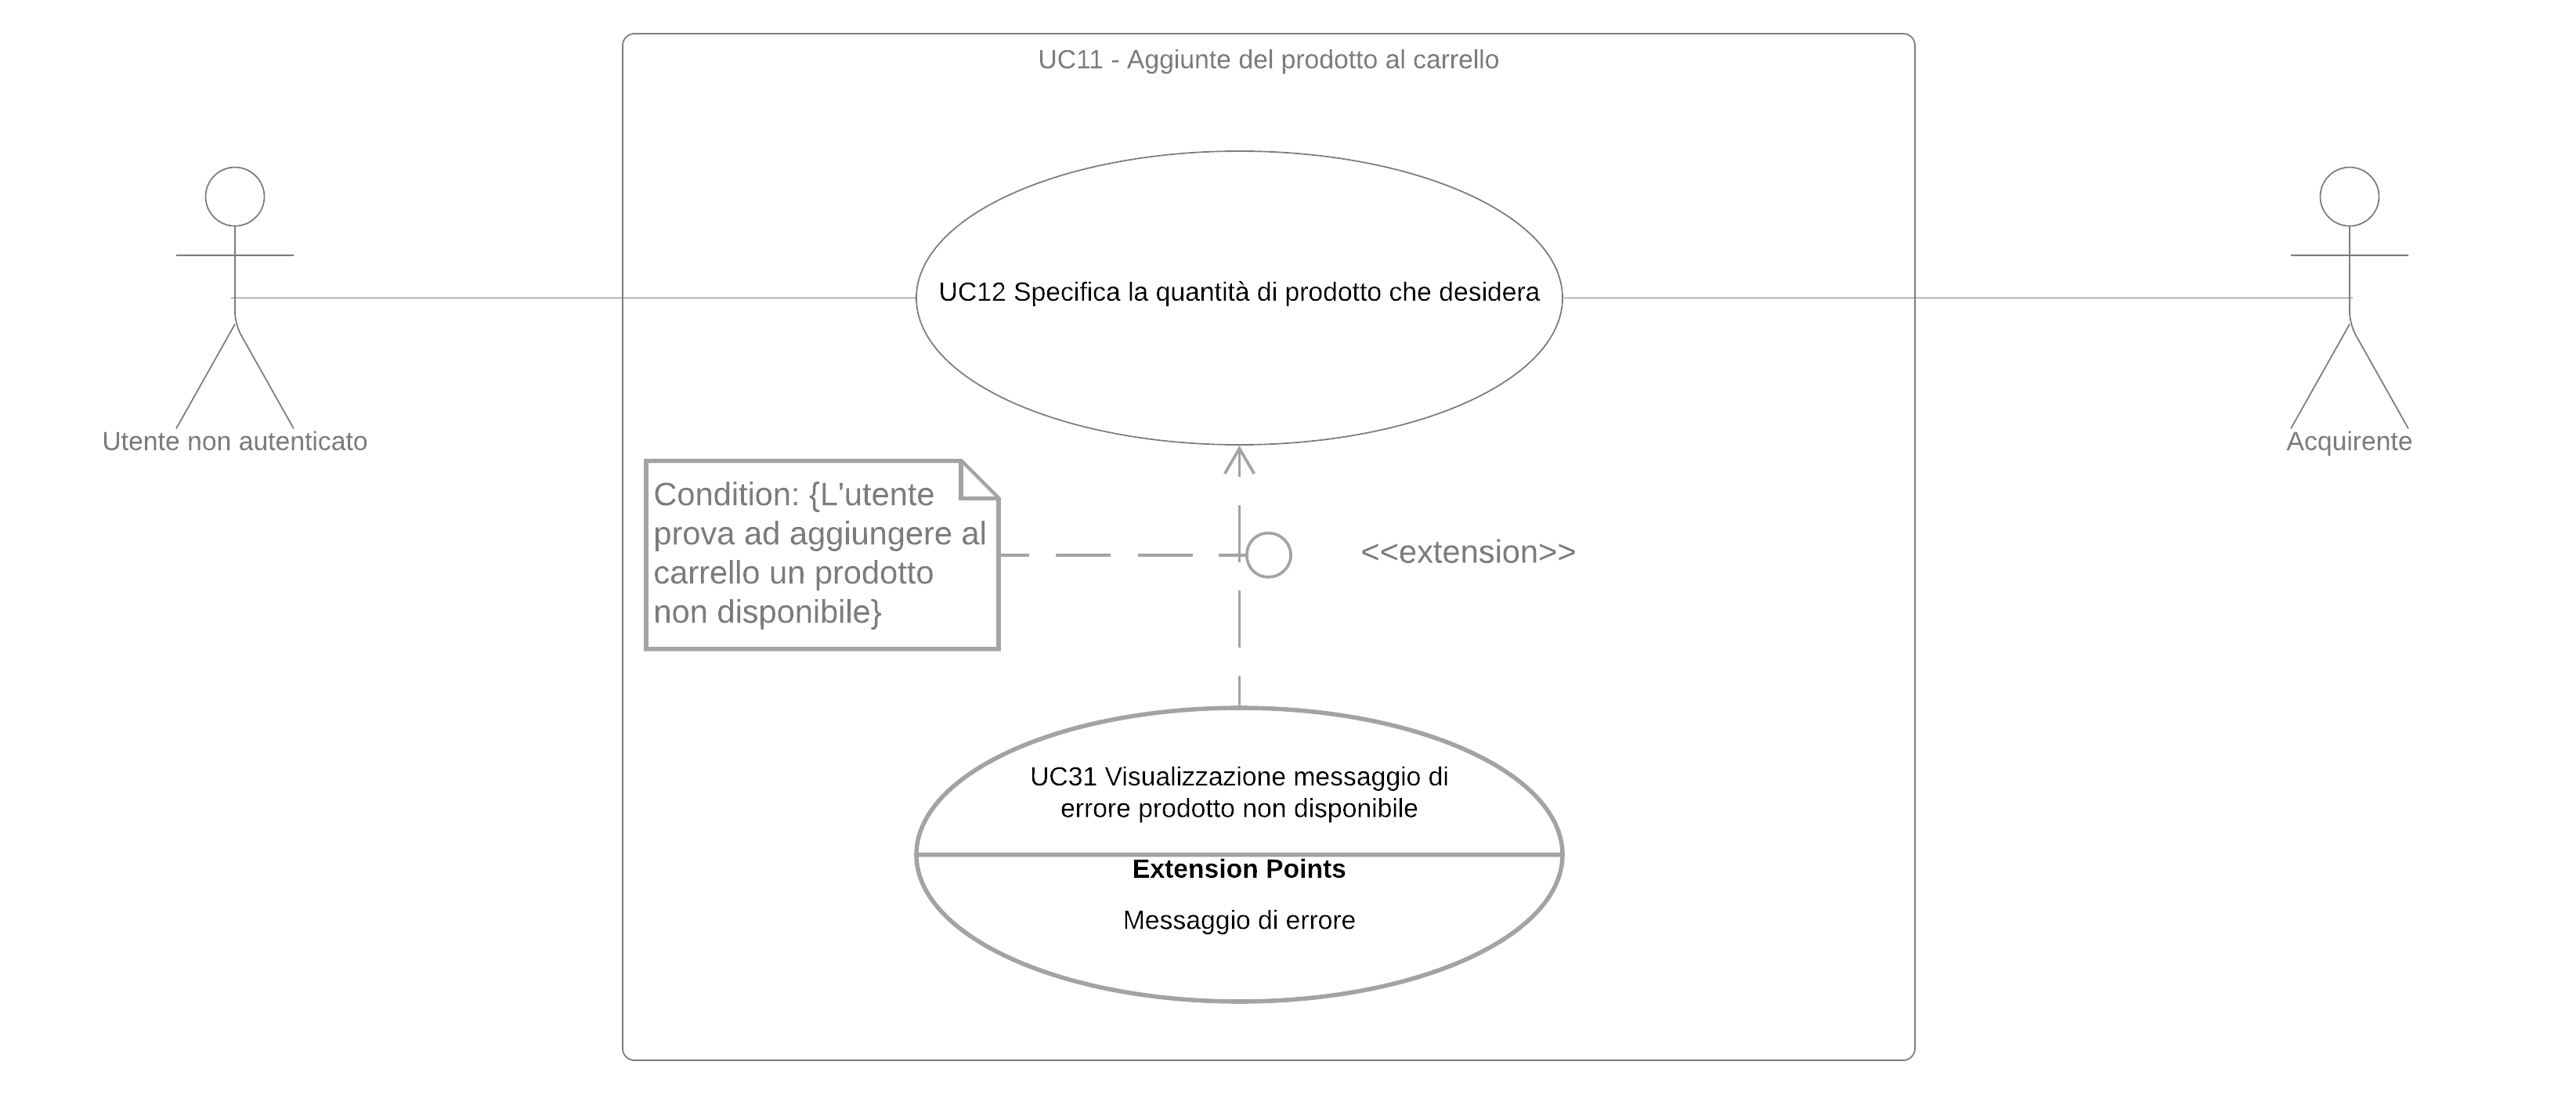
\includegraphics[width=\textwidth]{Immagini/DiagrammiUC/UC11AggiuntaProdottoAlCarrello.png}
%     \caption{Diagramma di \actualUC: Aggiunta del prodotto al carrello}
%     \label{fig:Checkout}
% \end{figure}

% L'utente non autenticato o l'acquirente può aggiungere al carrello i prodotti.
% \begin{itemize}
%     \item \textbf{Attori Primari:} Acquirente; Utente non autenticato
%     \item \textbf{Precondizione:} L'attore richiede di aggiungere una certa quantità del prodotto al carrello. 
%     \item \textbf{Postcondizione:} L'attore ha aggiunto la quantità desiderata di prodotto al carrello.
%     \item \textbf{Scenario Principale:} 
%     \begin{itemize}
%         \item (UC12) - Specifica la quantità di prodotto che desidera.
%         \item L'attore aggiunge il prodotto al carrello.
%         \item Il suo carrello personale viene aggiornato con il nuovo prodotto nella quantità indicata.
%     \end{itemize}
% \end{itemize}

%%%%%%%%%%%%%%%%%%%%%%%%%%%%%%%%%%%%%%%%%%%%%%%%%%%%%%%%%%%%%%%%%%%%%%%%%%%%%%%%%%%%%%%%%%%%%%%%%%%%%%%%%%%%%%%%%%%%%%%%%%%%%%%%%%%%%%%%%%%%%%%%%%%%%%%%%%%%%%%%%%%%%%%%%%%%%%

\UC{Modifica della quantità di un prodotto nel carrello}
L'acquirente o l'utente non autenticato modifica la quantità del prodotto già nel carrello.
\begin{itemize}
    \item \textbf{Attori primari:} acquirente o utente non autenticato;
    \item \textbf{Precondizione:} l'attore ha inserito un prodotto nel carrello e desidera modificarne la sua quantità;
    \item \textbf{Postcondizione:} la quantità del prodotto inserito nel carrello è aggiornata;
    \item \textbf{Scenario Principale:}
        \begin{itemize}
            \item l'attore aumenta o diminuisce la quantità tra 1 e la disponibilità massima di prodotto;
            \item la nuova quantità di prodotto sarà quella fornita.
        \end{itemize}
\end{itemize}

%%%%%%%%%%%%%%%%%%%%%%%%%%%%%%%%%%%%%%%%%%%%%%%%%%%%%%%%%%%%%%%%%%%%%%%%%%%%%%%%%%%%%%%%%%%%%%%%%%%%%%%%%%%%%%%%%%%%%%%%%%%%%%%%%%%%%%%%%%%%%%%%%%%%%%%%%%%%%%%%%%%%%%%%%%%%%%

\UC{Checkout}
\begin{figure}[H]
    \centering
    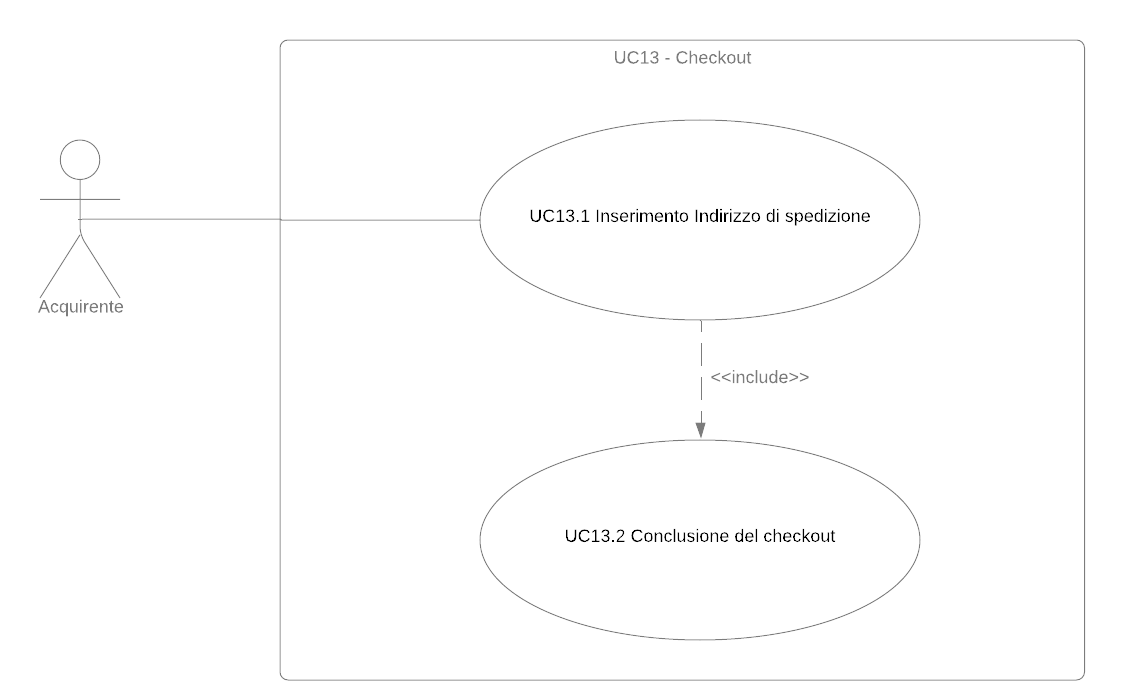
\includegraphics[scale=0.4]{Immagini/DiagrammiUC/UC13Checkout.png}
    \caption{Diagramma di \actualUC: Checkout} 
    \label{fig:Checkout}
\end{figure}

L'utente si trova nella pagina del carrello e vuole procedere al checkout per acquistare i prodotti scelti.
\begin{itemize}
    \item \textbf{Attori primari:} utente non autenticato o acquirente;
    \item \textbf{Attori secondari:} stripe;
    \item \textbf{Precondizione:} l'attore si trova nella pagina del carrello;
    \item \textbf{Postcondizione:} l'attore ha terminato il checkout e visualizza il riepilogo ordine.
    \item \textbf{Scenario principale:} l'attore si trova nella pagina del carrello, seleziona la funzionalità per procedere con il checkout. In seguito farà i seguenti passi:
    \begin{itemize}
    	\item Sceglie l'indirizzo di spedizione, in particolare esegue una delle seguenti azioni: 
    	\begin{itemize}
    		\item Selezionare l'indirizzo di spedizione precedentemente inserito;
    		\item (UC) - Inserire un nuovo indirizzo di spedizione.
    	\end{itemize}
    	\item Sceglie la carta per il pagamento, in particolare esegue una delle seguenti azioni: 
    	\begin{itemize}
    		\item Selezionare la carta da utilizzare precedentemente inserita;
    		\item (UC) - Inserire una nuova carta;
    	\end{itemize}
        \item (UC) - Invia il pagamento.
    \end{itemize}
    \item \textbf{Scenario alternativo 1:} Se l'attore non è ancora autenticato, viene reindirizzato alla login (UC1.2) o alla schermata per la registrazione per autenticarsi come acquirente, per poi procedere al checkout.
    \item \textbf{Scenario alternativo 2:} Se l'utente non autenticato è stato reindirizzato alla login e accede come venditore, il carrello con i prodotti salvati viene svuotato.
\end{itemize}

\resetSubUC

\subUC{Inserimento indirizzo di spedizione}
L'acquirente inserisce l'indirizzo al quale verrà spedito il pacco con l'ordine effettuato.
\begin{itemize}
    \item \textbf{Attori Primari:} Acquirente.
    \item \textbf{Precondizione:} Acquirente non ha ancora inserito l'indirizzo di spedizione.
    \item \textbf{Postcondizione:} Acquirente ha inserito l'indirizzo di spedizione e vengono calcolati e mostrati il costo della spedizione e i dazi doganali.
    \item \textbf{Scenario Principale:}
    \begin{itemize}
        \item (UC23.4) - L'acquirente inserisce l'indirizzo di spedizione obbligatorio.
        \item Vengono calcolati i costi di spedizione e i dazi doganali.
        \item Vengono mostrati i costi aggiuntivi appena calcolati.
        \item Dopo aver accettato anche i costi aggiuntivi, verrà reindirizzato alla pagina di Stripe.
    \end{itemize}
    \item \textbf{Estensioni:}
    \begin{itemize}
        \item (UC30) - Visualizzazione messaggio indirizzo di spedizione non inserito.
    \end{itemize}
\end{itemize}

\subUC{Invio del pagamento}
L'acquirente procede al pagamento attraverso il servizio fornito da Stripe e poi gli viene mostrata una pagina con il resoconto dell'ordine.
\begin{itemize}
    \item \textbf{Attori primari:} acquirente e Stripe;
    \item \textbf{Precondizione:} l'acquirente non ha ancora pagato e il carrello non è vuoto;
    \item \textbf{Postcondizione:} l'acquirente ha effettuato il pagamento, il suo carrello è vuoto e si trova sulla pagina di riepilogo dell'ordine;
    \item \textbf{Scenario principale:}
        \begin{itemize}
            \item l'acquirente viene indirizzato alla pagina di checkout di Stripe, dove pagherà il costo del carrello più le spese di spedizione e le tasse;
            \item Stripe si occupa del pagamento;
            \item Quando è avvenuto il pagamento viene svuotato il carrello e gli articoli che lo componevano vengono sottratti nella quantità acquistata da quelli disponibili;
            \item Viene visualizzato il riepilogo ordine.
        \end{itemize}
    \item \textbf{Scenario alternativo:} Se il pagamento fallisce l'utente viene riportato alla pagina del carrello, senza che questo venga svuotato.
\end{itemize}

%%%%%%%%%%%%%%%%%%%%%%%%%%%%%%%%%%%%%%%%%%%%%%%%%%%%%%%%%%%%%%%%%%%%%%%%%%%%%%%%%%%%%%%%%%%%%%%%%%%%%%%%%%%%%%%%%%%%%%%%%%%%%%%%%%%%%%%%%%%%%%%%%%%%%%%%%%%%%%%%%%%%%%%%%%%%%%

\UC{Visualizzazione riepilogo ordini in gestione}
Il venditore vuole vedere gli ordini gestiti o da gestire.
\begin{itemize}
    \item \textbf{Attori primari:} venditore;
    \item \textbf{Precondizione:} il venditore da qualsiasi schermata in cui si trovi vuole visualizzare gli ordini da gestire/gestiti;
    \item \textbf{Postcondizione:} Viene aperta la pagina di riepilogo ordini;
    \item \textbf{Scenario principale:}
    \begin{itemize}
        \item L'attore seleziona la funzione per visualizzare il riepilogo degli ordini in gestione;
        \item Viene indirizzato alla schermata con tutti gli ordini a suo carico, per ogni ordine sono indicati i prodotti acquistati, la quantità e l'indirizzo di spedizione.
    \end{itemize}
\end{itemize}
